\chapter{Building a Hexapod Model}

\section{Introduction to Control}
Control deals with how to move a limb into a desired state. Limbs and joints are
affected by forces. The effects of the forces must be carefully managed to
achieve the desired positioning of the limb or rotation of the joint. In humans
and animals motor control is a behaviour learned over time. Some techniques
attempt to emulate the learning process using techniques such as neural
networks, genetic algorithms or support vector machines
\cite{FaloutsosvandePanneTerzopolous, RusselSmith, Sims}. Other techniques attempt to
emulate the motion by studying the motion of the object in real life. 

\section{Previous Work}
A number of researchers have adopted the approach of using a learning algorithm
to achieve some form of control. Sanders et al. \cite{SandersLobbRiddle}
developed a series of 2 dimensional mass spring system based creatures. These
creatures, a biped like structure and a worm, produced locomotion by
contracting and expanding the virtual muscles that were modelled using spring
forces. The training of the controllers was accomplished using an evolutionary
algorithm.  Grzeszczuk et al. \cite{GrzeszczukTerzopoulos} present a technique
that synthesizes realistic locomotion of physics based animal models that are
highly flexible and have many degrees of freedom, such as a snake or dolphin.
The underlying assumption is that locomotion is an inherintly energy efficient
behaviour. This allows an objective function to be defined.  Optimal control
methods are able to minimize the objective function over a time interval.
Controllers are repeatedly generated and their effectiveness at producing
locomotion is evaluated. The controller set generated is a multilevel
controller that can handle complex locomotion because it is based on low level
controllers that optimize muscle actuation. Smith \cite{RusselSmith} developed
an extension to the CMAC neural network and applied it to train the motion
controller of a bipedal robot. Faloutsos et al. \cite{FaloutsosvandePanneTerzopolous} 
discuss composition of controllers and use support vector machines to
decide when to apply a controller. There is no discussion related to the
definition of the controllers. A radical example of learning control is shown
by Grzeszczuk et al \cite{GrzeszczukTerzopoulosHinton} where the physics based
models are replaced with a neural network that emulates that physics. In other
words, not only is the control learned, but so is the physics.  This approach
has the advantage of being less computationally demanding than a true
physics-based simulation that numerically solves the equations of motion. An
interesting approach was adopted by Sims \cite{Sims} where the morphology (i.e.
the shape) of the creature and the controller for locomotion was evolved
using genetic algorithms. Different fitness functions are used to direct guide
creatures to specific behaviours, such as swimming or walking.

Using a learning algorithm is not the only way to develop a motion controller.
For example Tu \cite{TuTerzopoulos} in her work on the motion of artificial
fishes, essentially hand coded the brain of the controller and via
experimentation found the optimal parameters for the controller. The fish was
modelled using a mass spring system. This allowed it to move through the water
by expanding an contracting opposing muscle groups.  A similar approach, based
on the observed motion of a real cockroach, was used by McKenna et al.
\cite{McKennaZeltzer}. The gait controller handles the timing of the steps of
the insect and is governed by a sinusoidal function. The motor controller is
responsible for creating the required force.  This force is passed to the
dynamics system, implemented using Featherstone's algorithm for articulated body
motion, that converts the forces into a meaningful positioning of the legs of
the insect. Panne et al. \cite{PanneLamouret} use a 'hand of God'
force to keep the character upright while it learnt how to walk or run. This
essentially means that a force was invented to allow the character to learn how
to stand. The idea is analogous to allowing training wheels on a bike or the
teaching of motor-control skills to people who need to learn how to walk again.
In \cite{GrzeszczukTerzopoulos} the authors note that this type of approach,
where the brain of the controller is programmed and parameters found via
experimentation can be a painstaking task requiring hours of experimentation.

\section{Environment}
The insect walks on a flat surface. A simple spring force proportional to the
penetration depth of a particle is created to simulate a hard surface. Friction
is modelled using a simple model relative to the one described by Baraff 
\cite{BaraffFriction}. The friction force is given by the following equation
when a particle is in contact with the ground and its velocity is greater than
0.
\[
\mathbf{F} = -k_d|\mathbf{F}_{perp}|\frac{\mathbf{v_{par}}}{|\mathbf{v_{par}}|}
\]
where $\mathbf{F}_{perp}$ is the force perpendicular to the plane and
$\mathbf{v}_{par}$ is velocity of the particle in the plane and $k_d$ is the
dynamic friction constant. The situation is illustrated in figure
\ref{Fig:Friction}.
\begin{figure}
    \centering
    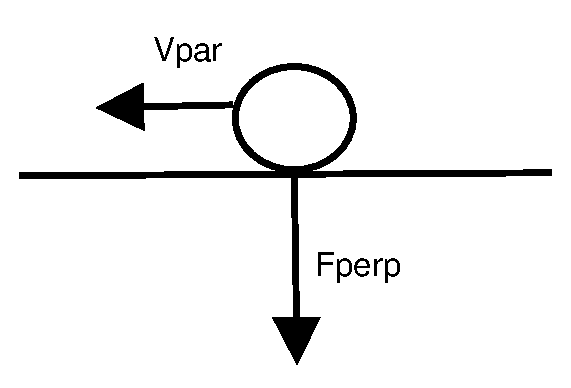
\includegraphics[height=0.125\textheight]{Friction}
    \caption{\label{Fig:Friction}Diagram showing some of the elements that make
    up the friction force.
    calculated.}
\end{figure}

\section{Attempts at Control}
The design or putting together of something that vaguely resembled a hexapod was
a fairly long process. Feedback from the simulation was gathered visually in
realtime. Running the simulation in debug mode was a problem since an
unoptimized build would run far too slowly to get any realtime feedback. Some
profiling done indicated that the majority of the time was spent doing matrix
multiplications for the equation \ref{Eqn:LambdaStable}. Solving that equation
using the biconjugate gradient solver took relatively less time.

We made heavy use fo fixed distance constraints and initially put togther the
hexapod shown in figure \ref{Fig:NoFixedAngle}. The creature is made up of 16
fixed distance constraints. The red balls represent particles. The creature in
the picture is falling over. This prompted the development of a fixed angle
constraint \ref{SubSec:FixedAngleConstraint} in order to keep the body of the
creature from twisting. These fixed angle constraints were added to the
creatures upper body.  The only problem was that adding more constraints slowed
down the simulation significantly. It became impossible to get any real time
feedback on what was going on even with the executable optimized
for speed.  So an effort had to be made to find a shape for the creature that
limited the number of constraints in order to get decent realtime response.
\begin{figure}
    \centering
    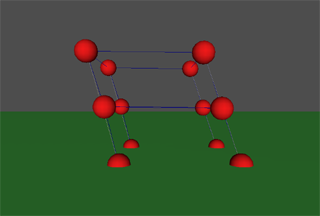
\includegraphics[height=0.25\textheight]{NoFixedAngle}
    \caption{\label{Fig:NoFixedAngle}An initial attempt. The picture shows the
    creature tilting towards the left. The blue lines between particles indicate
    a fixed distance constraint. The lack of any fixed angle constraints caused
    it to be unstable.}
\end{figure}

The creature was redesigned as shown in figure \ref{Fig:InsectThing0}. In this
case standing was achieved by setting a target position that the particle had to
satisfy. Changing target positions allowed the particles to move to those
positions. In this way the hexapod could lift its legs as shown in figure
\ref{Fig:InsectThing1}. The problem with this approach is that it is too similar
to keyframe, or more specifically procedural, animation. In procedural animation
the positions of the particles are keyframed by a function like sine. This
case, where the target position induces a force on the particle, is
analogous to keyframing the accelerations of the particles.
\begin{figure}
    \centering
    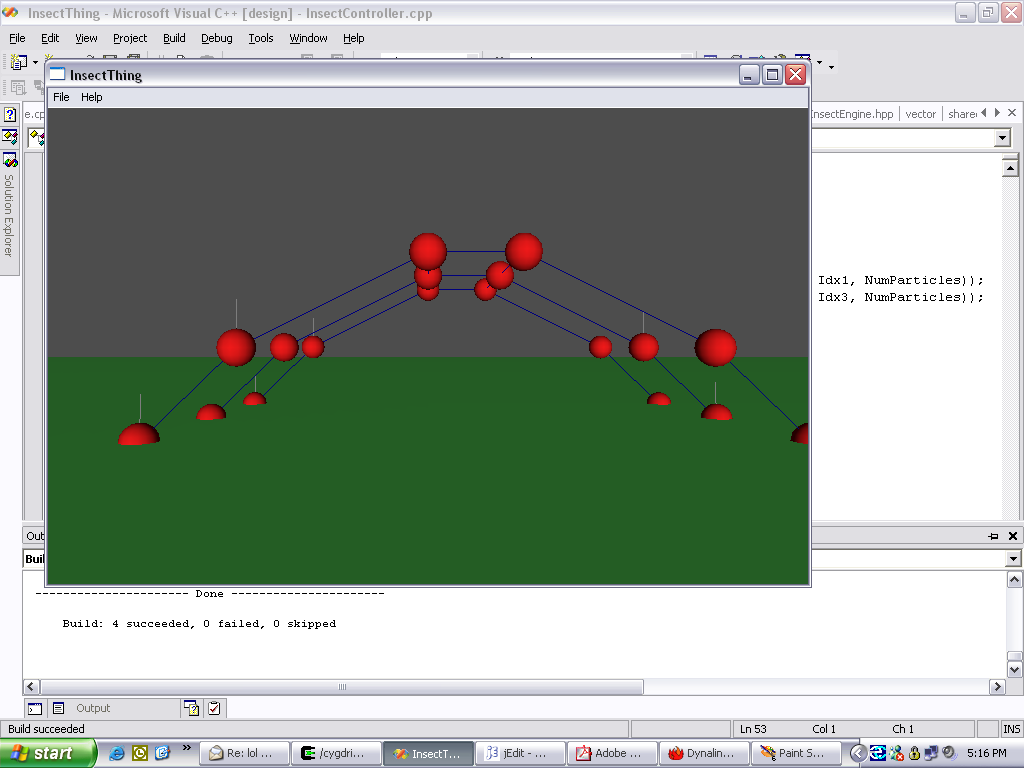
\includegraphics[height=0.5\textheight]{InsectThing1}
    \caption{\label{Fig:InsectThing0}The hexapod standing on six legs. The white
    lines represent target positions of the particles.}
\end{figure}
\begin{figure}
\centering
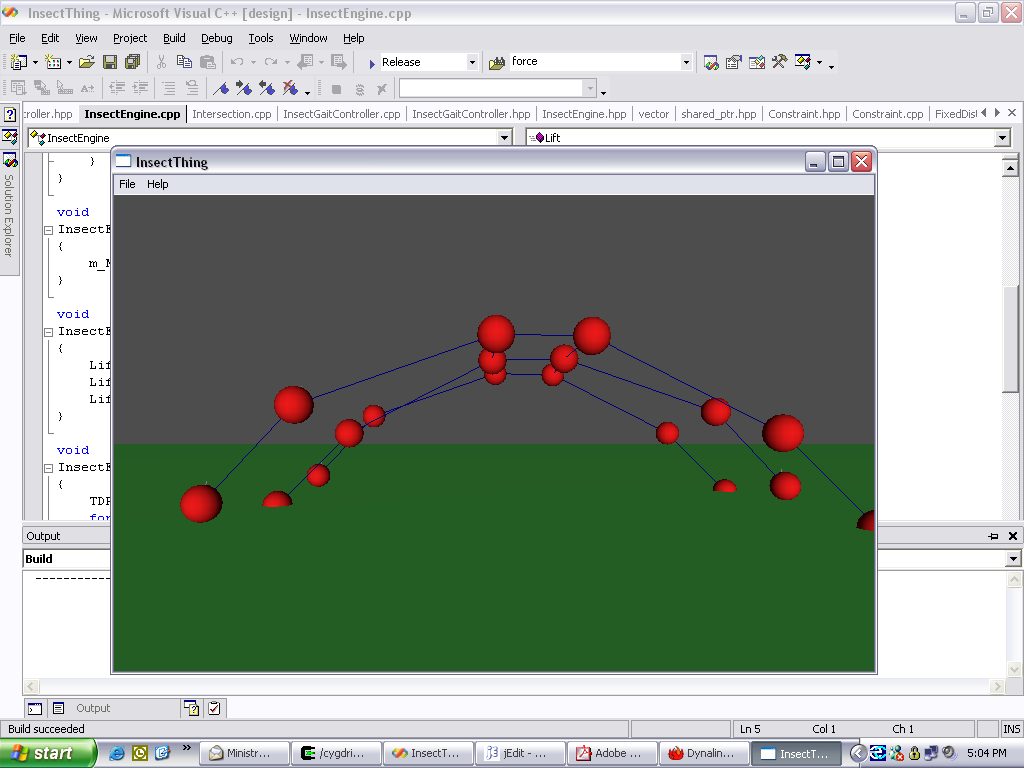
\includegraphics[height=0.5\textheight]{InsectThing0}
\caption{\label{Fig:InsectThing1}The hexapod standing on three legs.}
\end{figure}

Another attempt at controlling the hexapod was made by trying to simulate joint
controllers. The figure \ref{Fig:JointSpring} illustrates the spring at the
joint. If the springs rest angle is not satisfied then forces are applied to
the surrounding particles. The formula for calculating the force on p2 is 
\[
\mathbf{F} = k(\theta_r - \theta)|\mathbf{u} \times (\mathbf{v} \times
\mathbf{u})|
\]
where $\theta_r$ is the rest angle and $\theta$ is the current angle between the
vectors $\mathbf{u}$ and $\mathbf{v}$ and $k$ is the spring constant.
Similarly, the formula for calculating the force on p0 is given by
\[
 \mathbf{F} = k(\theta_r - \theta)|\mathbf{v} \times (\mathbf{v} \times
 \mathbf{u})|
\]
\begin{figure}
\centering
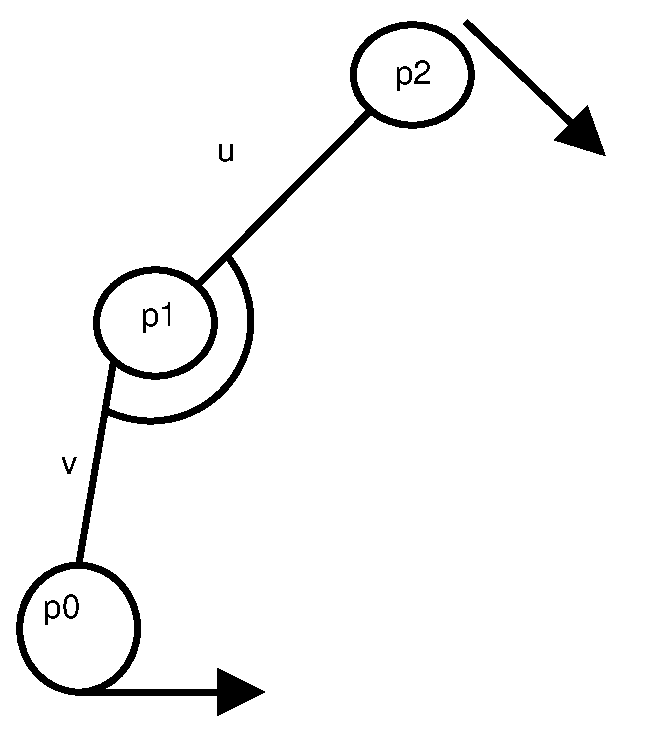
\includegraphics[height=0.25\textheight]{JointSpring}
\caption{\label{Fig:JointSpring}The hexapod joint.} 
\end{figure}
This configuraton allowed the hexapod to stand provided the spring constant was
sufficiently strong. The figure \ref{Fig:JointStiffness1} shows the hexapod
collapsing under the weight of its body because the stiffness of the joint was
not strong enough to support it. The hexapod also collapsed when the joint
stiffness was 10 as shown in figure \ref{Fig:JointStiffness10}. It took a joint
stiffness of 100 to prevent it collapsing \ref{Fig:StableJointStiffness100}.
\begin{figure}
\centering
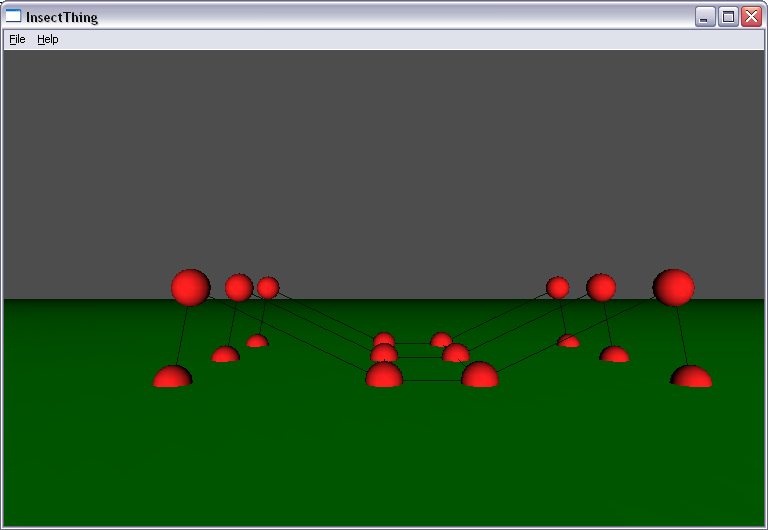
\includegraphics[height=0.5\textheight]{JointStiffness1}
\caption{\label{Fig:JointStiffness1}The hexapod collapsing under its own weight. The
joint stiffness was 1.} 
\end{figure}
\begin{figure}
\centering
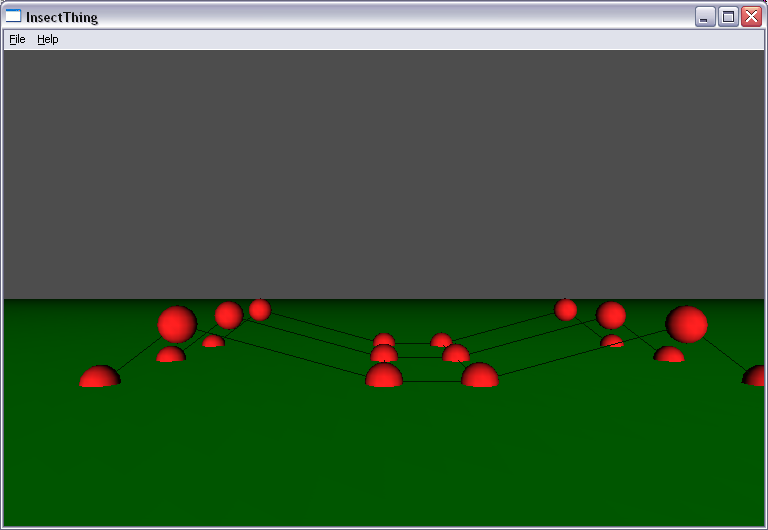
\includegraphics[height=0.5\textheight]{JointStiffness10}
\caption{\label{Fig:JointStiffness10}The hexapod collapsing under its own weight. The
joint stiffness was 10.} 
\end{figure}
\begin{figure}
\centering
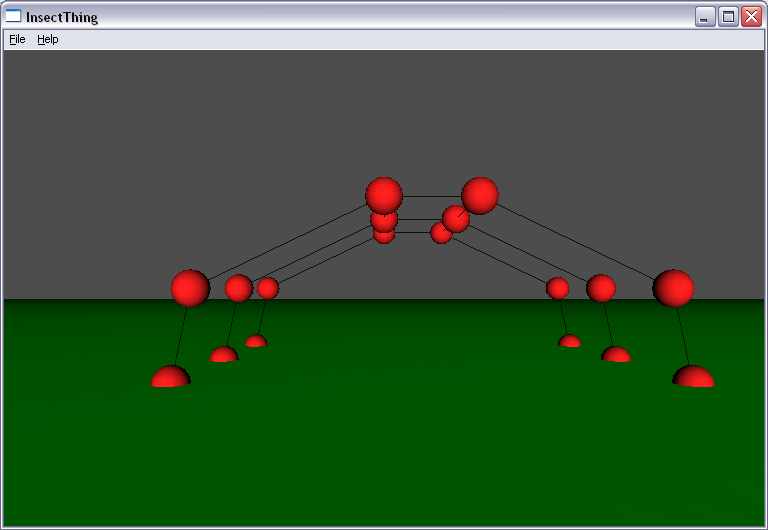
\includegraphics[height=0.5\textheight]{StableJointStiffness100}
\caption{\label{Fig:StableJointStiffness100}The hexapod standing. The
joint stiffness was 100.} 
\end{figure}

